\documentclass{article}[18pt]
\usepackage[utf8]{inputenc}
\usepackage[margin=0.7in]{geometry}
\usepackage{parselines} 
\usepackage{amsmath}
\usepackage{titlesec}

\usepackage{pgfplots}
\pgfmathdeclarefunction{gauss}{2}{%
  \pgfmathparse{1/(#2*sqrt(2*pi))*exp(-((x-#1)^2)/(2*#2^2))}%
}

\usepackage{graphicx}
\usepackage[english]{babel}
\usepackage{fancyhdr}
\usepackage{gensymb}
\usepackage{amssymb}
\usepackage{tabularx}
\pgfplotsset{width=10cm,compat=1.9}
\usepackage{tikz}
\usetikzlibrary{shapes.geometric, arrows}
\tikzstyle{startstop} = [rectangle, rounded corners, minimum width=3cm, minimum height=1cm,text centered, draw=black, fill=red!30]
\tikzstyle{io} = [trapezium, trapezium left angle=70, trapezium right angle=110, minimum width=3cm, minimum height=1cm, text centered, draw=black, fill=blue!30]
\tikzstyle{process} = [rectangle, minimum width=3cm, minimum height=1cm, text centered, draw=black, fill=orange!30]
\tikzstyle{decision} = [diamond, minimum width=3cm, minimum height=1cm, text centered, draw=black, fill=green!30,text width=2cm]
\tikzstyle{arrow} = [thick,->,>=stealth]

\titlespacing\section{0pt}{14pt plus 4pt minus 2pt}{0pt plus 2pt minus 2pt}
\newlength\tindent
\setlength{\tindent}{\parindent}
\setlength{\parindent}{0pt}
\renewcommand{\indent}{\hspace*{\tindent}}

\pagestyle{fancy}
\fancyhf{}
\rhead{Sam Robbins 13SE}
\lhead{A Level Maths - S2}
\rfoot{Page \thepage}


\begin{document}
\begin{center}
\underline{\huge Hypothesis testing}
\end{center}
\section{Performing a hypothesis test}
{\renewcommand{\arraystretch}{2}
\begin{tabularx}{\textwidth}{|X|X|}
\hline
Method&Example\\
\hline
\textbf{Establish the null and alternative hypothesis} \newline($H_0$ and $H_1$)&$H_0:p=0.5$\newline$H_1:p>0.5$\\
\hline
\textbf{Define the distribution under $\mathbf{H_0}$}&Under $H_0$ $X\sim B(15,0.5)$\\
\hline
\textbf{Decide on the significance level}&$5\%$\\
\hline
\textbf{Collect data, state the test statistic}&X=12\\
\hline
\textbf{Calculate the probability of obtaining the test statistic or a more extreme result}&
\begin{tabular}{r l}
$P(X\geqslant 12)$&$=1-P(X\leqslant 11)$\\
&$=1-0.9824$\\
&$=0.0176$\\
\end{tabular}
\\
\hline
\textbf{Compare this to the sig level as a decimal}&$0.0176<0.05$\\
\hline
\textbf{Interpret the results in terms of the original claim}&
There is evidence to reject $H_0$ in favour of $H_1$. The test is significant.\\
\hline
\end{tabularx}}
\section{Finding the critical region}
\begin{tikzpicture}
\begin{axis}[
  no markers, domain=0:8, samples=100,
  every axis y label/.style={at=(current axis.above origin),anchor=south},
  every axis x label/.style={at=(current axis.right of origin),anchor=west},
  height=5cm, width=12cm,
  xtick={2,6},xticklabels={5\%,95\%}, ytick=\empty,
  enlargelimits=false, clip=false,   ]
  \addplot [fill=cyan!20, draw=none, domain=0:2] {gauss(4,1)} \closedcycle;
  \addplot [fill=cyan!20, draw=none, domain=6:8] {gauss(4,1)} \closedcycle;
  \addplot [very thick,cyan!50!black] {gauss(4,1)};
\end{axis}
\end{tikzpicture}
\\
If the test statistic is found in the critical region $H_0$ will be rejected
\subsection{Finding the Lower critical value}
$P(X\geqslant c)<0.95$\\
$1-P(X\leqslant c-1)<0.95$\\
$\mathbf{P(X\leqslant c-1)>0.05}$
\subsection{Finding the Upper critical value}
$P(X\geqslant c)<0.05$\\
$1-P(X\leqslant c-1)<0.05$\\
$\mathbf{P(X\leqslant c-1)>0.95}$
\\
\\
\textbf{Then look these up in tables to find the critical values}



\newpage
\begin{center}

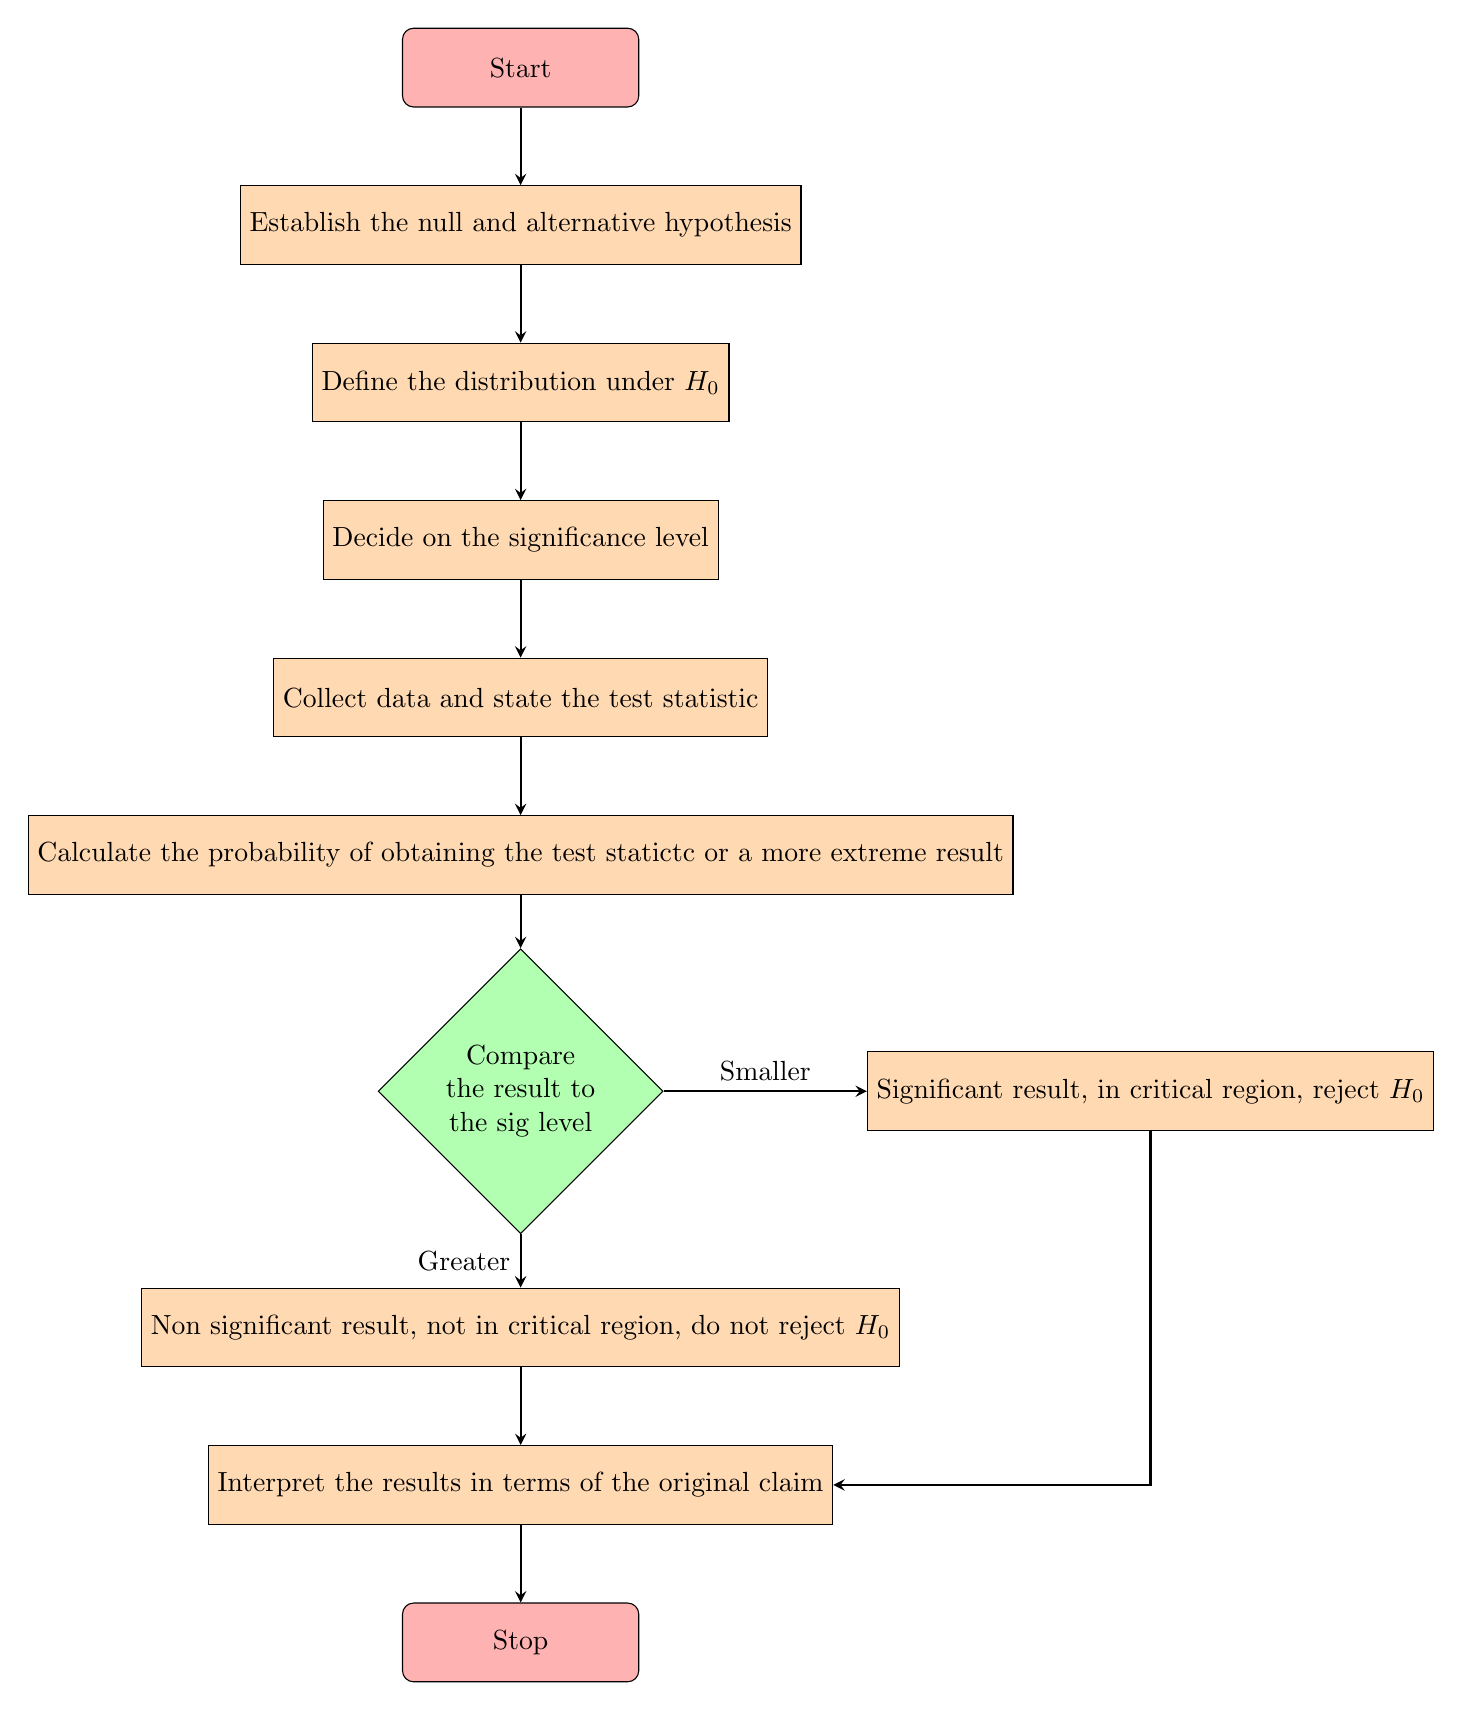
\begin{tikzpicture}[node distance=2cm]
\node (start) [startstop] {Start};
\node (pro1) [process, below of=start] {Establish the null and alternative hypothesis};
\node (pro2) [process, below of=pro1] {Define the distribution under $H_0$};
\node (pro3) [process, below of=pro2] {Decide on the significance level};
\node (pro4) [process, below of=pro3] {Collect data and state the test statistic};
\node (pro5) [process, below of=pro4] {Calculate the probability of obtaining the test statictc or a more extreme result};
\node (dec1) [decision, below of=pro5, yshift=-1cm] {Compare the result to the sig level};
\node (pro6) [process, below of=dec1,yshift=-1cm] {Non significant result, not in critical region, do not reject $H_0$};
\node (pro7) [process, right of=dec1,xshift=6cm] {Significant result, in critical region, reject $H_0$};
\node (pro8) [process, below of=pro6] {Interpret the results in terms of the original claim};
\node (stop) [startstop, below of=pro8] {Stop};

\draw [arrow] (start) -- (pro1);
\draw [arrow] (pro1) -- (pro2);
\draw [arrow] (pro2) -- (pro3);
\draw [arrow] (pro3) -- (pro4);
\draw [arrow] (pro4) -- (pro5);
\draw [arrow] (pro5) -- (dec1);
\draw [arrow] (dec1) -- node[anchor=east] {Greater} (pro6);
\draw [arrow] (dec1) -- node[anchor=south] {Smaller} (pro7);
\draw [arrow] (pro6) -- (pro8);
\draw [arrow] (pro7) |- (pro8);
\draw [arrow] (pro8) -- (stop);
\end{tikzpicture}

\end{center}
\end{document}